% \section{Demonstration}

Da die Implementierung nun erfolgt und beschrieben ist, wird nun beispielhaft der Nutzen dessen vorgestellt. Auf Basis der eingebauten Fehlerszenarien in der Demoanwendung soll der Mehrwert der erstellten Lösung evaluiert werden. Folgend wird näher beleuchtet, wie die drei Fehlerszenarien aufgedeckt werden können.

\subsection{Aufdecken des Szenarios \enquote{Keine Übersetzungen}}

In diesem Fehlerszenario sind für den Nutzer in der Webanwendung die Übersetzungsschlüssel zu sehen, statt der tatsächlichen Produktnamen (vgl. \autoref{subsec:keine-uebersetzungen}). Da es sich hierbei um einen Fallback handelt, wurde in der Webanwendung darauf verzichtet einen Fehler zu werfen. Dieser würde in Splunk hervorgehoben werden. Jedoch lassen sich in Splunk die Logdaten durchsuchen und so Sitzungen herausfinden, bei denen dieses Problem aufgetreten ist (vgl. \autoref{fig:keine-uebersetzungen_splunk-logs}). Darauf basierend konnten verwandte Logs der selben \enquote{Sitzung} inspiziert werden, jedoch konnte anhand dessen das Fehlverhalten nicht weiter nachvollzogen werden. Jedoch bietet die nun gefundene \texttt{shoppingCartId} die Möglichkeit, damit in weiteren Systemen nachzuforschen.
	
\begin{figure}[H]
	\centering
	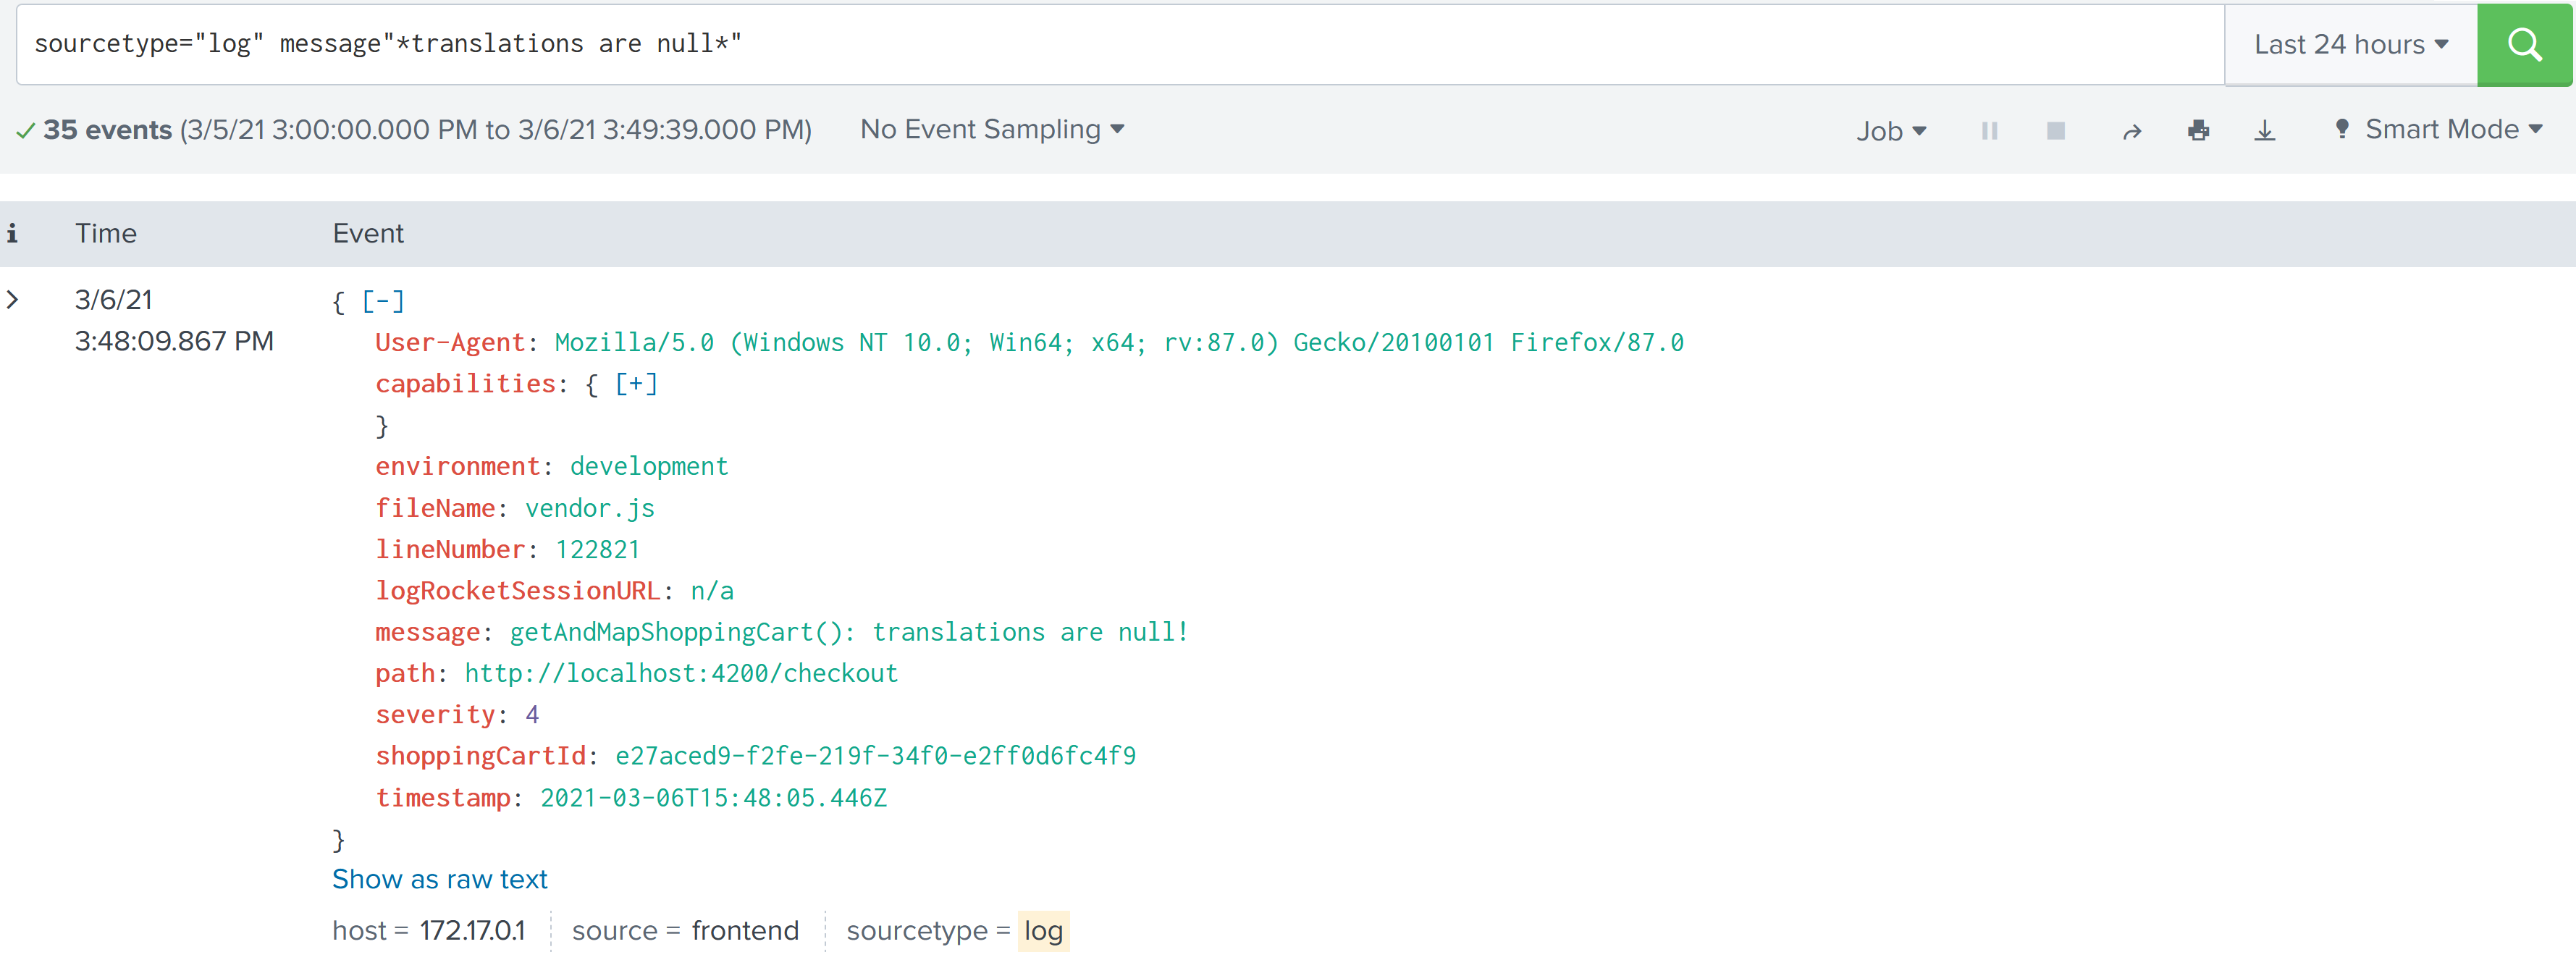
\includegraphics[width=1.00\linewidth]{img/05_ergebnis/keine-uebersetzungen_splunk-logs.png}
	\caption{Suche nach Logs zu fehlenden Übersetzungen in Splunk}
	\label{fig:keine-uebersetzungen_splunk-logs}
\end{figure}

\begin{wrapfigure}[13]{r}{0.50\textwidth}
\centering
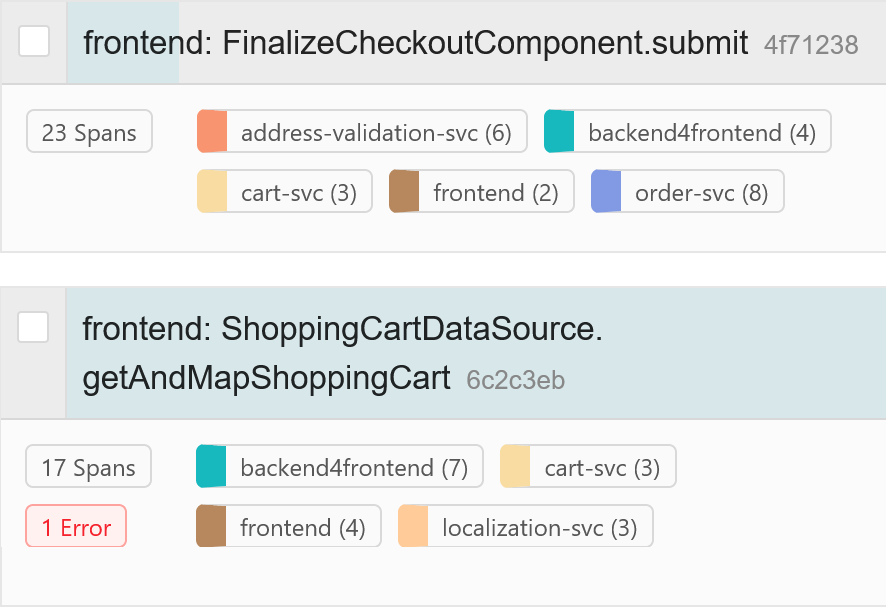
\includegraphics[width=\linewidth]{img/05_ergebnis/keine-uebersetzungen_jaeger_search-cropped.png}
\caption{Suchergebnisse in Jaeger zu spezieller \texttt{shoppingCartId}}
\label{fig:uebersetzungen_jaeger_search-cropped}
\end{wrapfigure}

In Jaeger lassen sich anhand der \texttt{shopping\-Cart\-Id} Traces finden (vgl. \autoref{fig:uebersetzungen_jaeger_search-cropped}). Einer dieser Traces ist mit einem Fehler markiert und entsprang der Funktion \texttt{getAndMapShoppingCart} im Frontend. Dabei handelt es sich um eine Funktion, die die Warenkorb- sowie Übersetzungsdaten abruft und diese zusammengeführt.

Bei Klick auf den Trace erhält man Einsicht in das entsprechende Trace-Gantt-Diagramm (vgl. \autoref{fig:keine-uebersetzungen_jaeger_detail}). Bei dem Aufruf ist im Übersetzungsdienst ein Fehler aufgetreten, welcher vermutlich die fehlenden Übersetzungen verursachte. Weiterhin wurde ein Log im Span hinterlegt, welches die genaue Ursache beschreibt: \texttt{configuration is invalid}. Zudem ist auch der genaue Kubernetes-Pod (\texttt{localization-svc-003}) zu sehen, der die Abfrage durchführte. Somit sind dem problemlösenden Entwickler viele notwendige Informationen geboten, die ihm dabei helfen das Problem zu lösen.

\begin{figure}[H]
	\centering
	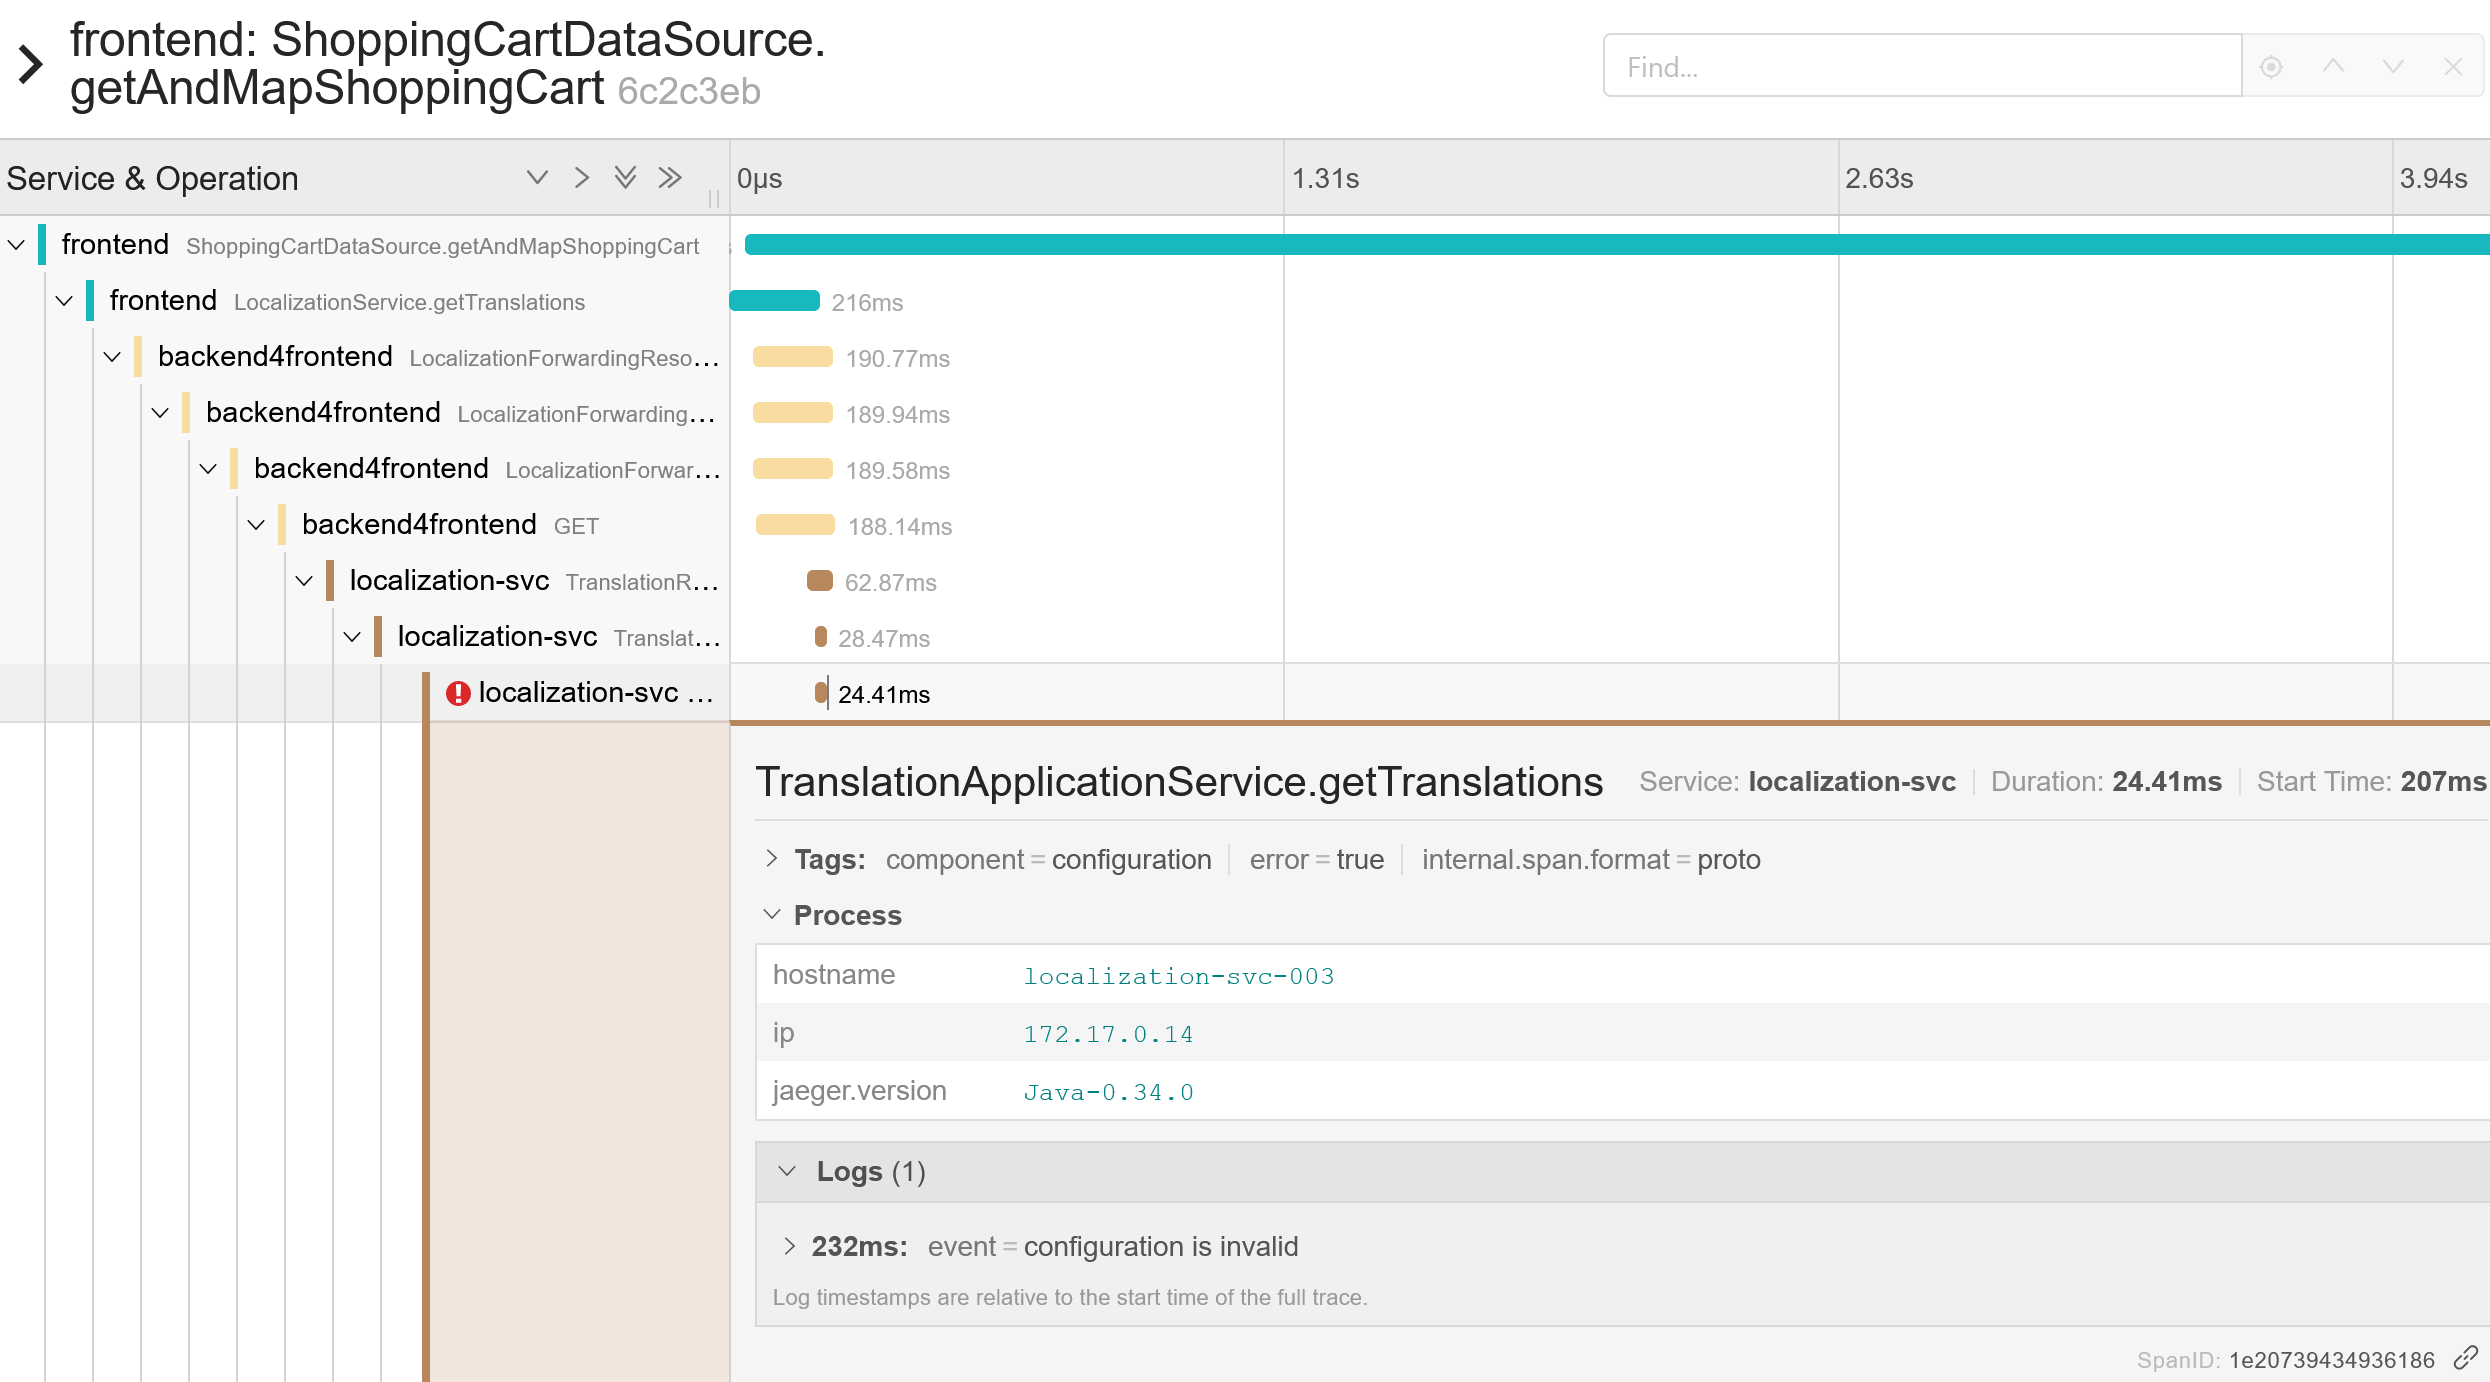
\includegraphics[width=1.00\linewidth]{img/05_ergebnis/keine-uebersetzungen_jaeger_detail.png}
	\caption{Auschnitt des Traces zur Übersetzungsanfrage in Jaeger}
	\label{fig:keine-uebersetzungen_jaeger_detail}
\end{figure}

\subsection{Aufdecken des Szenarios \enquote{Ungültige Adressen sind gültig}}

Das Backend bietet die Möglichkeit, dass die SPA eingegebene Adresse zuvor validiert. Bei der Rechnungs- sowie der Lieferadresse sollte dies auch der Fall sein. Jedoch kommt es dazu, dass Nutzer ungültige Adresse angeben können und dies bei der Aufgabe einer Bestellung zu einem Fehler führt (vgl. \autoref{subsec:ungueltige-adressen-sind-gueltig}). Durch die Suche in Splunk nach Logmeldungen der Angular-Komponente \texttt{Finalize\-Checkout\-Component} findet sich eine Fehlermeldung und eine entsprechende \texttt{shopping\-Cart\-Id}.

Bis auf die Fehlermeldung liefert Splunk jedoch nicht sprechende Informationen, deshalb wird erneut auf Jaeger zurückgegriffen. In Jaeger findet ein entsprechender Trace (vgl. \autoref{fig:ungueltige-adressen-sind-gueltig_jaeger-detail}), der über die Situation Aufschluss gibt. Es ist dabei zu erkennen, dass im Bestelldienst beide Adressen erneut validiert werden und dabei die Anfrage bzgl. der Lieferadresse fehlschlägt. Auf Basis dieser Informationen kann nun der Entwickler feststellen, dass in der SPA keine Validierung für die Lieferadresse durchgeführt wird.

\begin{figure}[H]
	\centering
	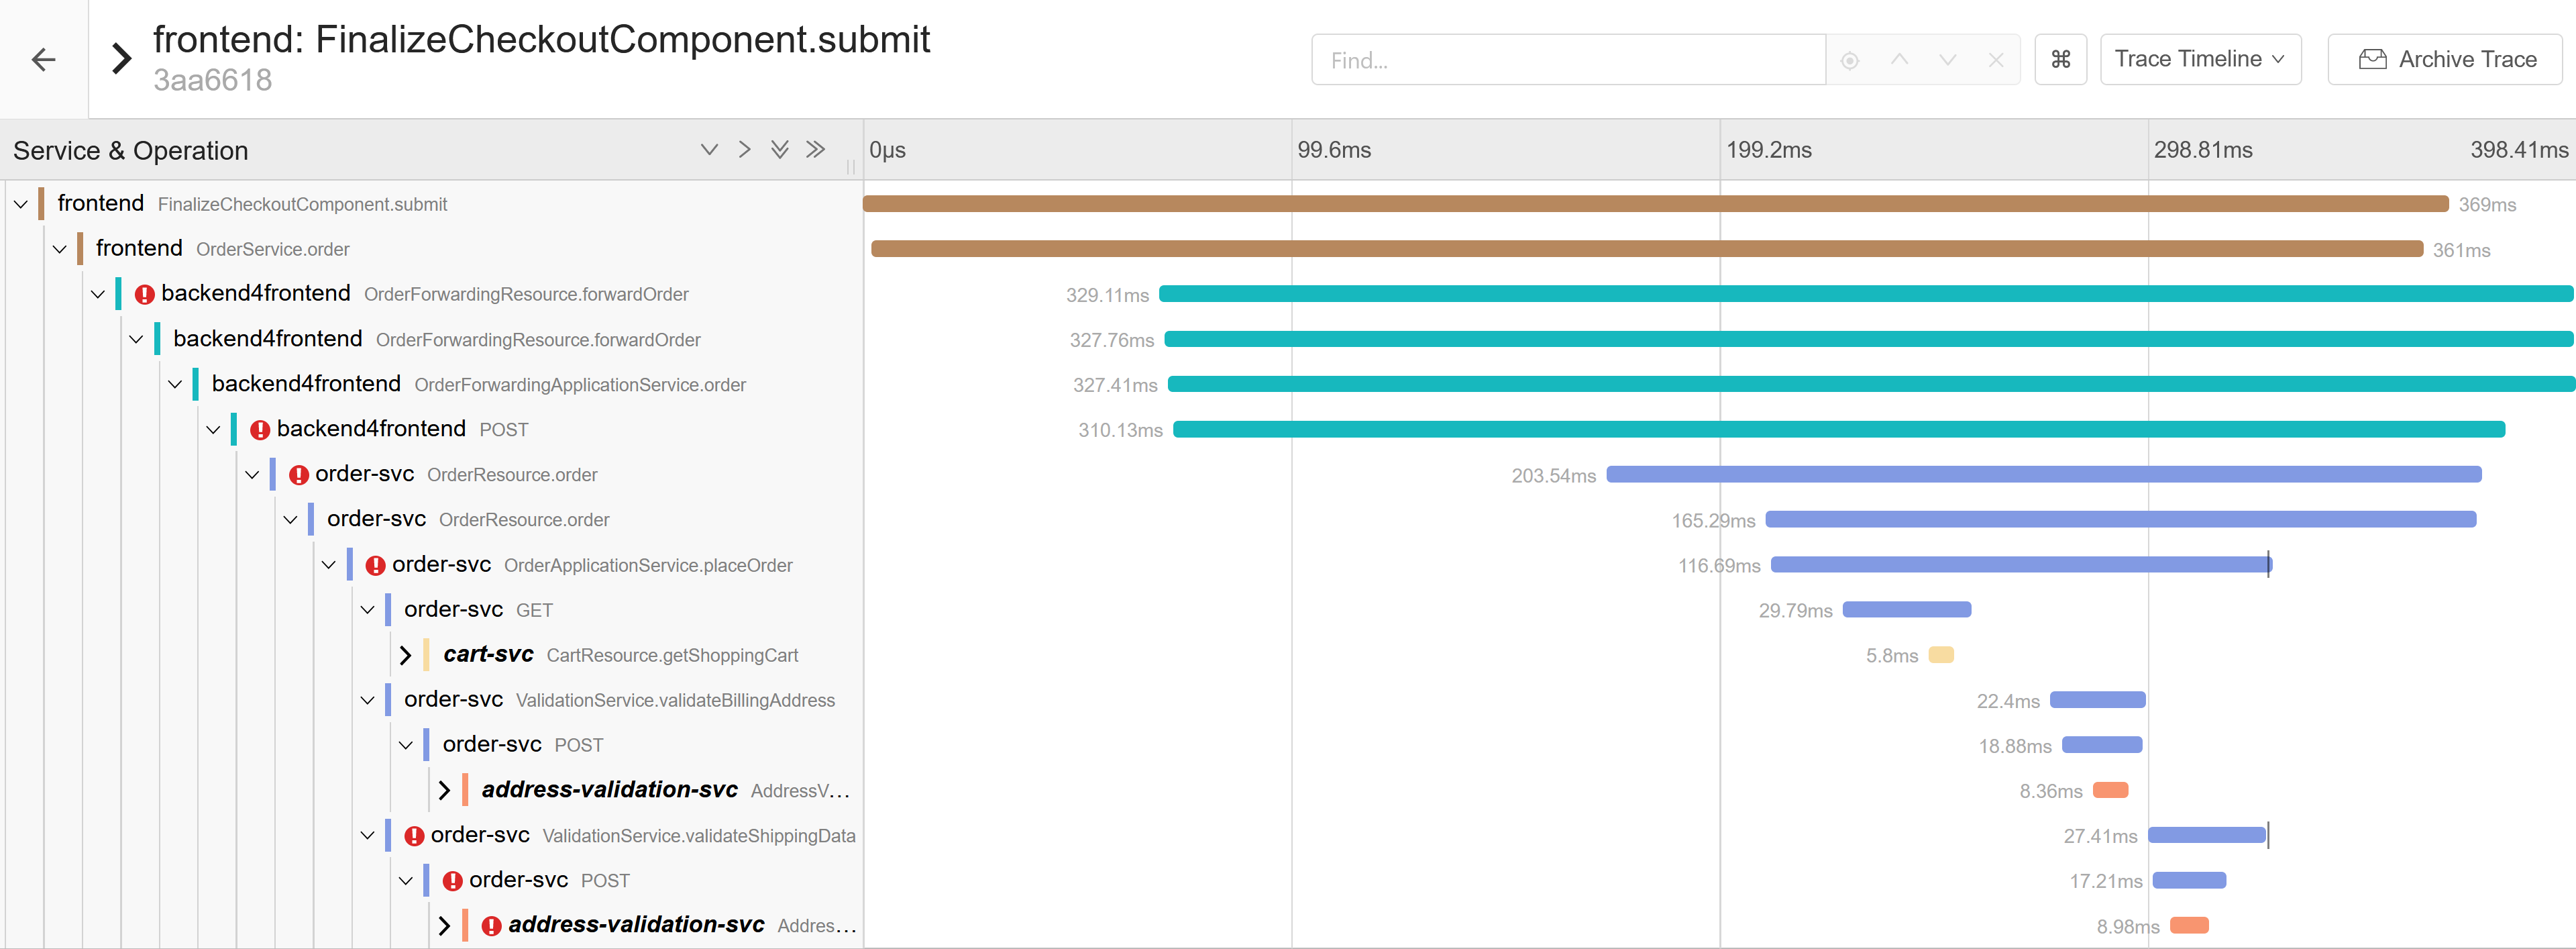
\includegraphics[width=1.00\linewidth]{img/05_ergebnis/ungueltige-adressen-sind-gueltig_jaeger-detail.png}
	\caption{Auschnitt des Traces zur Bestellanfrage in Jaeger}
	\label{fig:ungueltige-adressen-sind-gueltig_jaeger-detail}
\end{figure}

\subsection{Aufdecken des Szenarios \enquote{Lange Verarbeitung}}

In diesem Szenario kommt es bei der Anzeige des Warenkorbes zu einer starken Verzögerung, bis dieser Sichtbar ist (vgl. \autoref{subsec:lange-verarbeitung}). Hierbei ist Splunk wenig hilfreich, da eine zeitliche Abfolge alleine durch Logs schwer nachvollziehbar ist. Durch LogRocket ist das resultierende Verhalten gut nachvollzuziehen und ein Video dessen ist im Anhang vorzufinden (siehe \autoref{sec:demo-logrocket}).

Hierbei hilft erneut Jaeger, denn durch Traces lassen sich nicht nur hierarchische Beziehungen nachvollziehen, sondern auch zeitliche. Eine Trace-Gantt-Visualisierung eines Traces, bei dem der Warenkorb abgerufen wird, ist in \autoref{fig:lange-verarbeitung_jaeger} zu betrachten. Dabei sticht hervor, dass der überwiegende Anteil der Zeit nicht in den Backendanfragen verloren geht, sondern durch die Operation \texttt{mapShoppingCart} im Frontend geschieht. Anhand dieser Informationen kann ein Entwickler nun hergehen und diese Operation verbessern.

\begin{figure}[H]
	\centering
	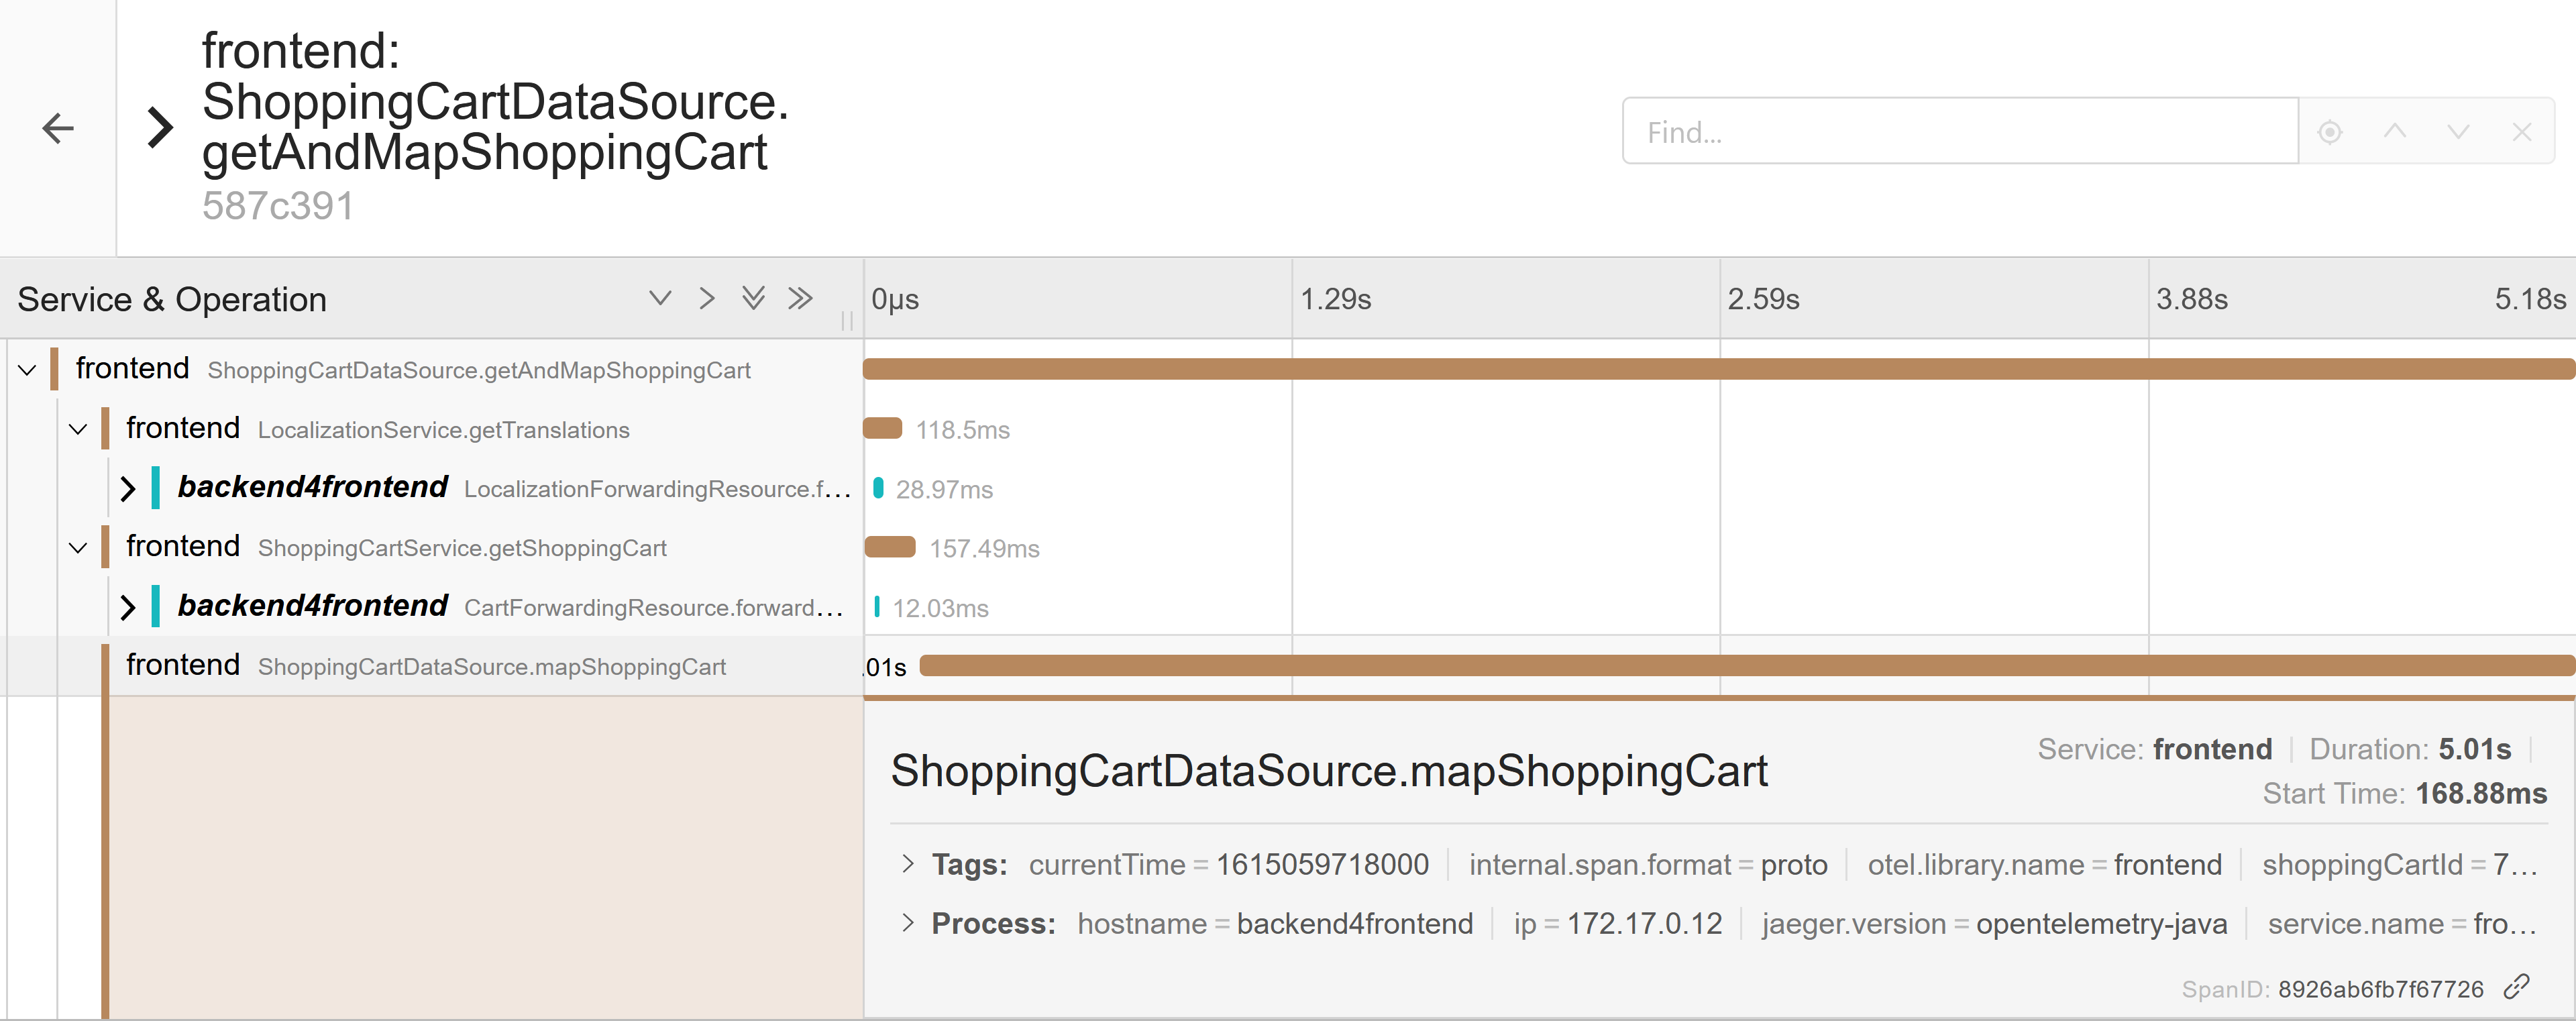
\includegraphics[width=1.00\linewidth]{img/05_ergebnis/lange-verarbeitung_jaeger.png}
	\caption{Auschnitt des Traces zur Warenkorbanfrage in Jaeger}
	\label{fig:lange-verarbeitung_jaeger}
\end{figure}